\documentclass[journal=jcisd8,manuscript=article]{achemso}

\usepackage[T1]{fontenc}
\usepackage{amsmath}
\usepackage{booktabs}
\usepackage{graphicx}

\newcommand*\mycommand[1]{\texttt{\emph{#1}}}
\renewcommand*\suppinfoname{Supporting Information}
\renewcommand*\tocentryname{For Table of Contents Only}
\newcommand{\TBD}[1]{\textbf{[#1]}}
\newcommand{\dS}{\Delta S}
\newcommand{\kcal}{kcal\,mol$^{-1}$}
\renewcommand{\topfraction}{0.9}
\renewcommand{\floatpagefraction}{0.7}
\setlength{\emergencystretch}{3em}
% Generated by make_numbers_docking.py; do not edit.
\newcommand{\dockAgreeBal}{0.93}
\newcommand{\dockAgreeDetail}{0.93}
\newcommand{\dockAgreeFast}{0.86}
\newcommand{\dockBillionDays}{810}
\newcommand{\dockBillionDaysFast}{270}
\newcommand{\dockPrepOkFourK}{4{,}093}
\newcommand{\dockRate}{14.3}
\newcommand{\dockRateFastest}{42.5}
\newcommand{\paramsPc}{848{,}002}
\newcommand{\paramsXa}{1{,}260{,}930}
\newcommand{\pocketDockDaysFast}{4.0}
\newcommand{\pocketPairs}{14.8}

\newcommand{\factorLabelShortlist}{3.9}
\newcommand{\hoConstTen}{0.79}
\newcommand{\hoDualTen}{0.79}
\newcommand{\hoGainDualTen}{0.00}
\newcommand{\hoGainDualTenHi}{0.02}
\newcommand{\hoGainDualTenLo}{$-$0.02}
\newcommand{\hoGainPooledTen}{$-$0.01}
\newcommand{\hoGainPooledTenHi}{0.00}
\newcommand{\hoGainPooledTenLo}{$-$0.03}
\newcommand{\hoGainXattnTen}{$-$0.04}
\newcommand{\hoGainXattnTenHi}{$-$0.01}
\newcommand{\hoGainXattnTenLo}{$-$0.07}
\newcommand{\hoNTargets}{49}
\newcommand{\hoPooledTen}{0.77}
\newcommand{\hoXattnTen}{0.75}
\newcommand{\kfConstTen}{0.81}
\newcommand{\kfConstTenHi}{0.85}
\newcommand{\kfConstTenLo}{0.76}
\newcommand{\kfDiffDualConstTen}{0.06}
\newcommand{\kfDiffDualConstTenHi}{0.10}
\newcommand{\kfDiffDualConstTenLo}{0.04}
\newcommand{\kfDiffPooledPooledConstTen}{0.08}
\newcommand{\kfDiffPooledPooledConstTenHi}{0.12}
\newcommand{\kfDiffPooledPooledConstTenLo}{0.05}
\newcommand{\kfDiffXattnDualTen}{0.04}
\newcommand{\kfDiffXattnDualTenHi}{0.06}
\newcommand{\kfDiffXattnDualTenLo}{0.03}
\newcommand{\kfDiffXattnXattnConstTen}{0.11}
\newcommand{\kfDiffXattnXattnConstTenHi}{0.15}
\newcommand{\kfDiffXattnXattnConstTenLo}{0.07}
\newcommand{\kfDualTen}{0.88}
\newcommand{\kfDualTenHi}{0.90}
\newcommand{\kfDualTenLo}{0.85}
\newcommand{\kfDualTwenty}{0.96}
\newcommand{\kfFoldTrainMax}{46}
\newcommand{\kfFoldTrainMin}{28}
\newcommand{\kfNTargets}{49}
\newcommand{\kfPooledTen}{0.89}
\newcommand{\kfPooledTenHi}{0.91}
\newcommand{\kfPooledTenLo}{0.87}
\newcommand{\kfRatioDual}{95}
\newcommand{\kfRatioDualHi}{97}
\newcommand{\kfRatioDualLo}{94}
\newcommand{\kfRatioDualLong}{97}
\newcommand{\kfRatioDualLongHi}{98}
\newcommand{\kfRatioDualLongLo}{96}
\newcommand{\kfRatioPooled}{97}
\newcommand{\kfXaBestHi}{54{,}846}
\newcommand{\kfXaBestLo}{42{,}658}
\newcommand{\kfXattnTen}{0.92}
\newcommand{\kfXattnTenHi}{0.93}
\newcommand{\kfXattnTenLo}{0.90}
\newcommand{\kfXattnTwenty}{0.98}
\newcommand{\kpConstTen}{0.83}
\newcommand{\kpDualTen}{0.86}
\newcommand{\kpNTargets}{39}
\newcommand{\kpSpreadTen}{0.01}
\newcommand{\kpXaBestHi}{18{,}282}
\newcommand{\kpXaBestLo}{12{,}188}
\newcommand{\kpXattnTen}{0.85}
\newcommand{\paramsDual}{848{,}002}
\newcommand{\shareLabelShortlist}{25}
\newcommand{\tmACpus}{96}
\newcommand{\tmADualFiftySevenFull}{43.3}
\newcommand{\tmADualPerPocketMs}{0.2}
\newcommand{\tmADualThousandFull}{43.5}
\newcommand{\tmAFeat}{39.3}
\newcommand{\tmAGpu}{RTX 4090}
\newcommand{\tmALig}{260{,}155}
\newcommand{\tmAPaddedHalf}{15}
\newcommand{\tmAPaddedSingle}{4.7}
\newcommand{\tmAProcs}{32}
\newcommand{\tmARatioXaHalfFiftySevenFull}{1.2}
\newcommand{\tmARatioXaHalfFiftySevenModel}{6.4}
\newcommand{\tmARatioXaHalfThousandFull}{4.5}
\newcommand{\tmARatioXaHalfThousandModel}{86}
\newcommand{\tmARatioXaSingleFiftySevenFull}{1.6}
\newcommand{\tmARatioXaSingleFiftySevenModel}{18}
\newcommand{\tmARatioXaSingleThousandFull}{12}
\newcommand{\tmARatioXaSingleThousandModel}{273}
\newcommand{\tmAXaHalfFiftySevenFull}{52.0}
\newcommand{\tmAXaHalfPerPocket}{0.15}
\newcommand{\tmAXaHalfThousandFull}{197}
\newcommand{\tmAXaSingleFiftySevenFull}{71.1}
\newcommand{\tmAXaSinglePerPocket}{0.49}
\newcommand{\tmAXaSingleThousandFull}{535}
\newcommand{\tmBCpus}{128}
\newcommand{\tmBFeat}{22.4}
\newcommand{\tmBGpu}{L40S}
\newcommand{\tmBPaddedHalf}{16}
\newcommand{\tmBPaddedSingle}{5.3}
\newcommand{\tmBProcs}{32}
\newcommand{\tmBRatioXaHalfFiftySevenFull}{1.4}
\newcommand{\tmBRatioXaHalfFiftySevenModel}{9.2}
\newcommand{\tmBRatioXaHalfThousandFull}{7.8}
\newcommand{\tmBRatioXaHalfThousandModel}{130}
\newcommand{\tmBRatioXaSingleFiftySevenFull}{2.2}
\newcommand{\tmBRatioXaSingleFiftySevenModel}{27}
\newcommand{\tmBRatioXaSingleThousandFull}{23}
\newcommand{\tmBRatioXaSingleThousandModel}{413}
\newcommand{\trainShareLib}{15.4}


\author{Hyunseung Kong}
\email{hskong@snu.ac.kr}
\affiliation{Interdisciplinary Program in Bioinformatics, Seoul National University, Seoul 08826, Republic of Korea}

\title{Jev-Like Shared-State Networks for Fast Structure-Based Screening}

\begin{document}

\begin{tocentry}
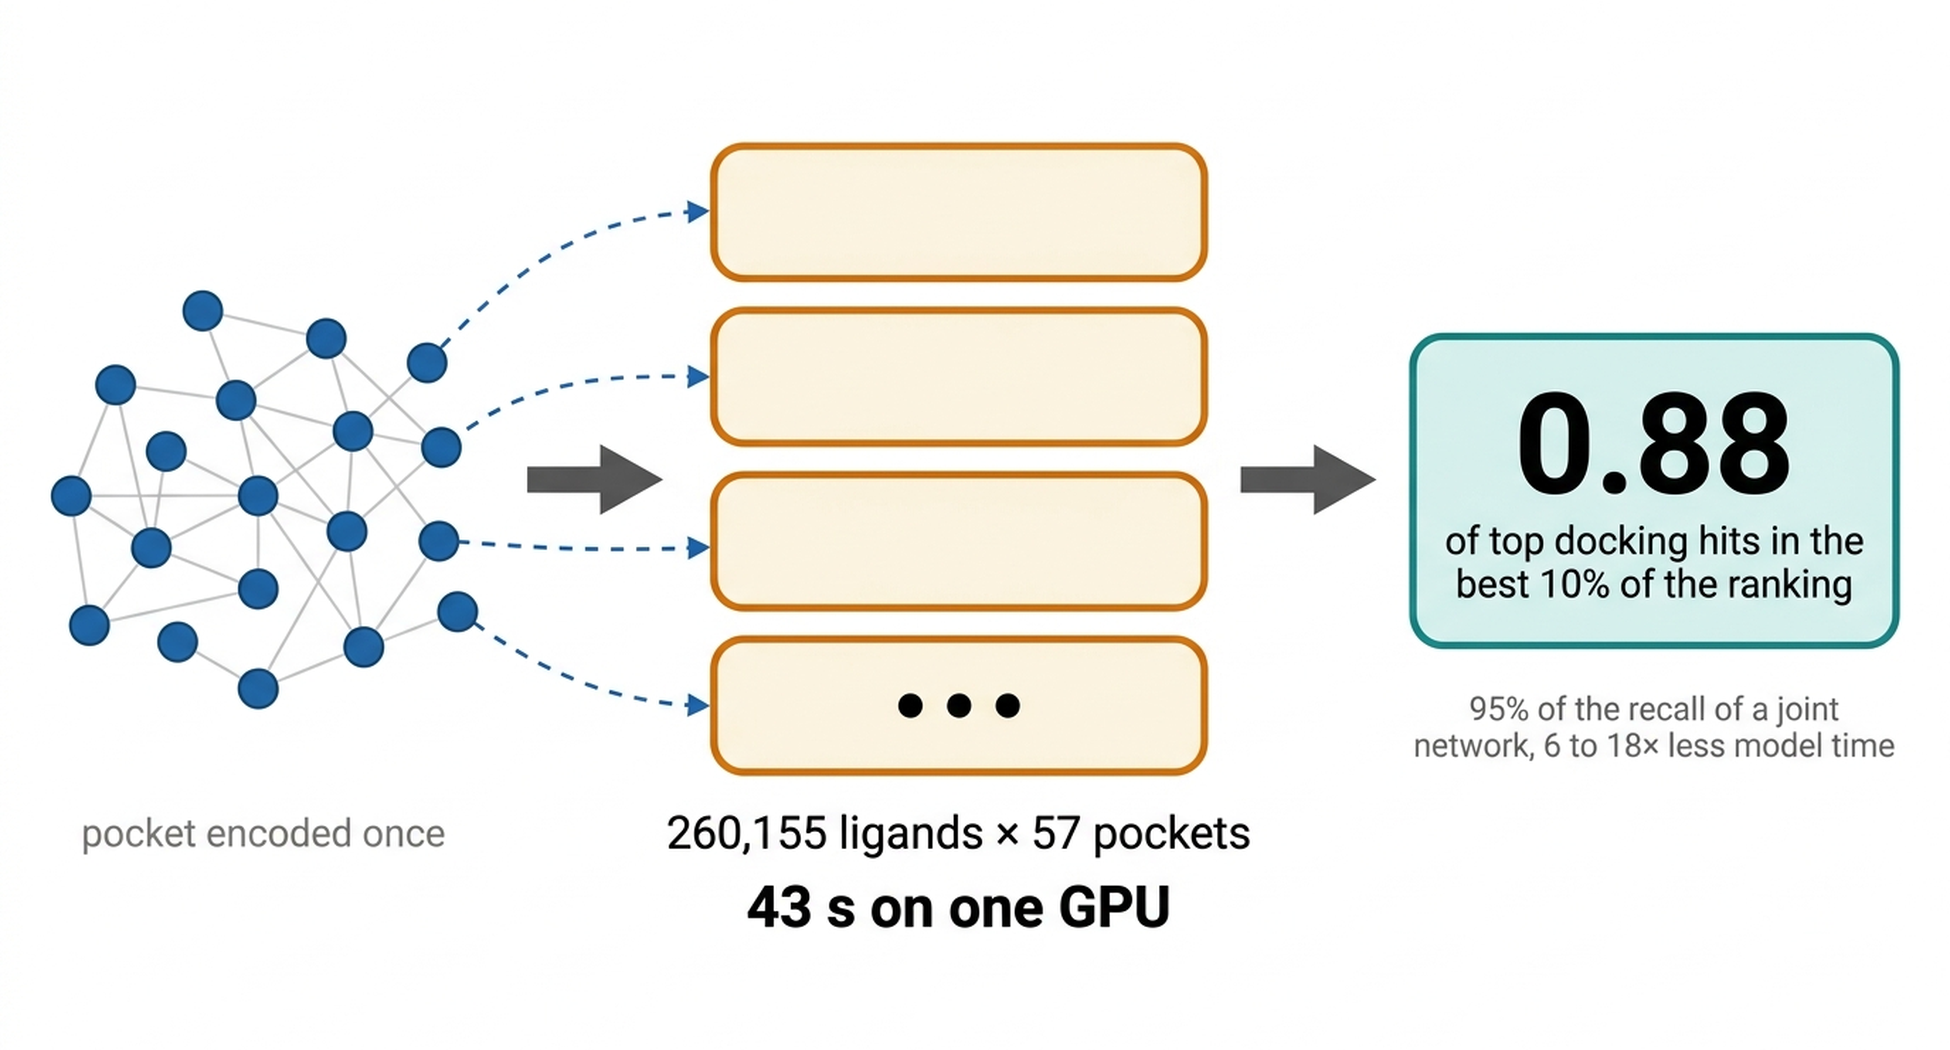
\includegraphics[width=\linewidth]{figures/toc.png}
\end{tocentry}

\begin{abstract}
Docking limits structure-based virtual screening: the fastest search mode of Uni-Dock needs \pocketDockDaysFast{} GPU-days for the \tmALig{} ligands of DOCKSTRING against 57 pockets. Neural surrogates trained on docking scores reduce this cost, but networks that let the ligand and the pocket interact before the readout, called joint networks here, pay for the interaction on every ligand-pocket pair. We built Jev-like networks, named after Jev of TypeSafe, that encode each pocket once into a shared state and embed each ligand independently of the pocket, so that a cheap readout scores every pair and the screen of a library against many pockets reduces to a matrix product. Trained on the docking scores of known pockets of DOCKSTRING and tested on new ligands for \kfNTargets{} of them, a Jev-like dual encoder recovers \kfDualTen{} of the top-1\% docking hits in the best 10\% of the ranking. A joint cross-attention network with the same encoders recovers \kfXattnTen{}, and a network that sees only the ligand \kfConstTen{}, so that the dual encoder keeps \kfRatioDual{}\% of the recall of the joint network. On one \tmAGpu{} the dual encoder ranks the ligands against 57 pockets from SMILES in \tmADualFiftySevenFull{} s and against 1{,}000 pockets in \tmADualThousandFull{} s, whereas the cross-attention network needs \tmARatioXaHalfThousandFull{} to \tmARatioXaSingleThousandFull{} times longer for 1{,}000 pockets in float16 and float32. A Jev-like network therefore keeps most of the recall of a joint network at a screening cost that hardly grows with the number of pockets, and docking only the best 10\% of its ranking costs a tenth of docking the library.
\end{abstract}

\section{Introduction}

Structure-based virtual screening ranks compounds by docking them into a protein pocket. Libraries of more than one hundred million molecules have been docked,\cite{lyu2019} an open-source platform has screened more than one billion compounds,\cite{gorgulla2020} and hierarchical schemes reach a library of eleven billion compounds by docking less than 0.1\% of it.\cite{sadybekov2022} Campaigns of this size are feasible on modest computer clusters,\cite{bender2021} multi-billion-scale collections of make-on-demand compounds are freely available,\cite{tingle2023} and the docking scores of the best molecules improve with the size of the library.\cite{lyu2023}

The docking calculation limits this scale. GPU engines accelerate AutoDock Vina\cite{vina,vina12} and AutoDock4,\cite{santosmartins2021} with reported speed-ups of more than 1{,}000-fold for Uni-Dock over one CPU core of AutoDock Vina\cite{unidock} and 65.6-fold on average for Vina-GPU 2.0 over AutoDock Vina in two DrugBank screens.\cite{vinagpu} In our measurements Uni-Dock docks \dockRate{} to \dockRateFastest{} ligands per second on one GPU at 4{,}000 ligands per call, depending on the search mode, which still puts a billion molecules at \dockBillionDaysFast{} to \dockBillionDays{} GPU-days for a single pocket.

Machine-learning surrogates cut this cost for a single target. Deep Docking, active learning and related workflows dock a sample of the library, fit a model to its scores and dock only the compounds that the model ranks first.\cite{deepdocking,gentile2022,molpal,yang2021,carlsson2025} On a library of 1.56 billion compounds, HASTEN recovered about 90\% of the 1{,}000 top-scoring molecules while docking 1\% of it,\cite{sivula2023} and regression-based active learning on libraries of one million molecules recovered up to 90\% of the top 1\% of the docking hits while docking 10\% of them.\cite{marin2024} Regressors on molecular fingerprints predict about 5{,}800 docking scores per second,\cite{berenger2021} and networks that emulate docking from the two-dimensional structure of the ligand run orders of magnitude faster than the docking program.\cite{jastrzebski2020} Benchmarks across targets and docking programs test these protocols,\cite{difilippo2025} and two reviews cover the field.\cite{sadybekov2023,cavasotto2023} Each of these models serves one target.

A surrogate that is trained on the docking scores of many pockets can serve all of them with one network, and its cost depends on where the network lets the ligand and the pocket meet. Many deep-learning scoring functions let them meet early. Convolutional networks read a three-dimensional grid of the protein-ligand complex,\cite{ragoza2017,stepniewska2018,francoeur2020} GNINA scores docked poses with an ensemble of such networks,\cite{gnina} graph networks model the interactions between ligand and protein atoms in three-dimensional complexes,\cite{jiang2021,moon2022,lai2024} and TransformerCPI lets the atoms of a compound attend to the protein in a transformer decoder.\cite{chen2020} KarmaDock accelerates the docking of large libraries,\cite{zhang2023} and EquiScore reaches high accuracy on screening test sets.\cite{cao2024} In these joint networks the representation of the ligand depends on the pocket, and every ligand-pocket pair passes through the interaction layers.

Jev, a model from TypeSafe, takes one state and several typed questions, evaluates the questions in parallel and in isolation against the same state, and returns all answers from a single query.\cite{jev,jevdocs} The public documentation does not describe the architecture behind this interface.\cite{jevdocs} We transfer the interface to screening, with the pocket as the state, the ligands as the questions and the scores as the answers (Figure~\ref{fig:concept}a). A surrogate of this organization encodes the pocket once into a state that stays in memory, embeds every ligand independently of the pocket and of the other ligands, and lets the ligand meet the pocket only at a cheap readout, so that a screen of a dual encoder against many pockets reduces to a product of two sets of vectors (Figure~\ref{fig:concept}b). We call such surrogates Jev-like. In the joint counterpart every ligand atom attends to the residues of the pocket in cross-attention layers (Figure~\ref{fig:concept}c).\cite{vaswani2017}

The same choice appears in text retrieval. Cross-encoders that read a query and a document together are accurate but too slow to rank a large collection, and bi-encoders that embed both independently allow the embeddings of the collection to be computed once.\cite{humeau2020} Finding the most similar pair among 10{,}000 sentences takes about 65 hours with BERT as a cross-encoder and about 5 seconds with sentence embeddings.\cite{reimers2019} ColBERT, a late-interaction ranker, precomputes the document representations offline and runs about two orders of magnitude faster than BERT rankers at competitive effectiveness,\cite{khattab2020} and dense dual encoders outperform sparse BM25 retrieval in open-domain question answering.\cite{karpukhin2020} The price is accuracy, since dual encoders trail cross-attention models,\cite{menon2022} and fixed-length vectors limit the precision of retrieval.\cite{luan2021}
Screening of protein-ligand pairs follows this path. DrugCLIP aligns pocket and molecule embeddings in a shared space and turns screening into retrieval,\cite{drugclip_arxiv,drugclip} CoSP pretrains pocket and ligand representations with a contrastive loss,\cite{gao2023} LigUnity learns a shared pocket-ligand space,\cite{ligunity2025} and DrugHash stores contrastively learned binary hash codes of the molecules.\cite{han2025} DrugCLIP is reported to run up to ten million times faster than docking and scored about 500 million compounds against 10,000 human proteins,\cite{drugclip} and PharmacoNet, which computes a pocket model once, scored 187 million compounds on a 32-core CPU in 21 hours and is reported to run 3,000 times faster than AutoDock Vina on PDBbind.\cite{pharmaconet} These speed-ups are measured against docking, and they leave open how much recall a shared pocket representation gives up against a joint network. Answering this needs the same encoders and the same training recipe on both sides, so that the networks differ only in the exchange of information between the ligand atoms and the pocket residues before the readout.

The study uses DOCKSTRING, which provides the docking scores of 260,155 ligands against 58 targets,\cite{dockstring} computed for every ligand-pocket pair, so that the hits of every pocket are known. The networks serve the pockets of their training data, the setting of a screen for which a docked sample of the library exists for every pocket of interest. Pockets outside the training data pose a different problem. Machine-learning scoring functions that predict binding for targets outside their training data exploit the biases of their data sets and lose accuracy on proteins and ligands that differ from the training data,\cite{chen2019,yang2020,volkov2022} and the benchmark accuracy of models trained on PDBbind rests largely on leakage of similar complexes between the training and test sets.\cite{graber2025}

We trained a dual encoder and a cross-attention network with the same encoders and the same recipe on the docking scores of the training pockets of DOCKSTRING\cite{dockstring} (Figure~\ref{fig:concept}) and evaluated them on new ligands for the pockets of their training data. A network with one constant dummy pocket marks the recall that the ligand alone supports, and a second Jev-like network with a learned readout tests whether the result depends on the product readout. We then measured the time that the networks need to screen the \pocketPairs{} million pairs of the library against 57 and 1{,}000 pockets on one \tmAGpu{} and compared it with the time that Uni-Dock needs to dock the same pairs.

\begin{figure}[t]
\centering
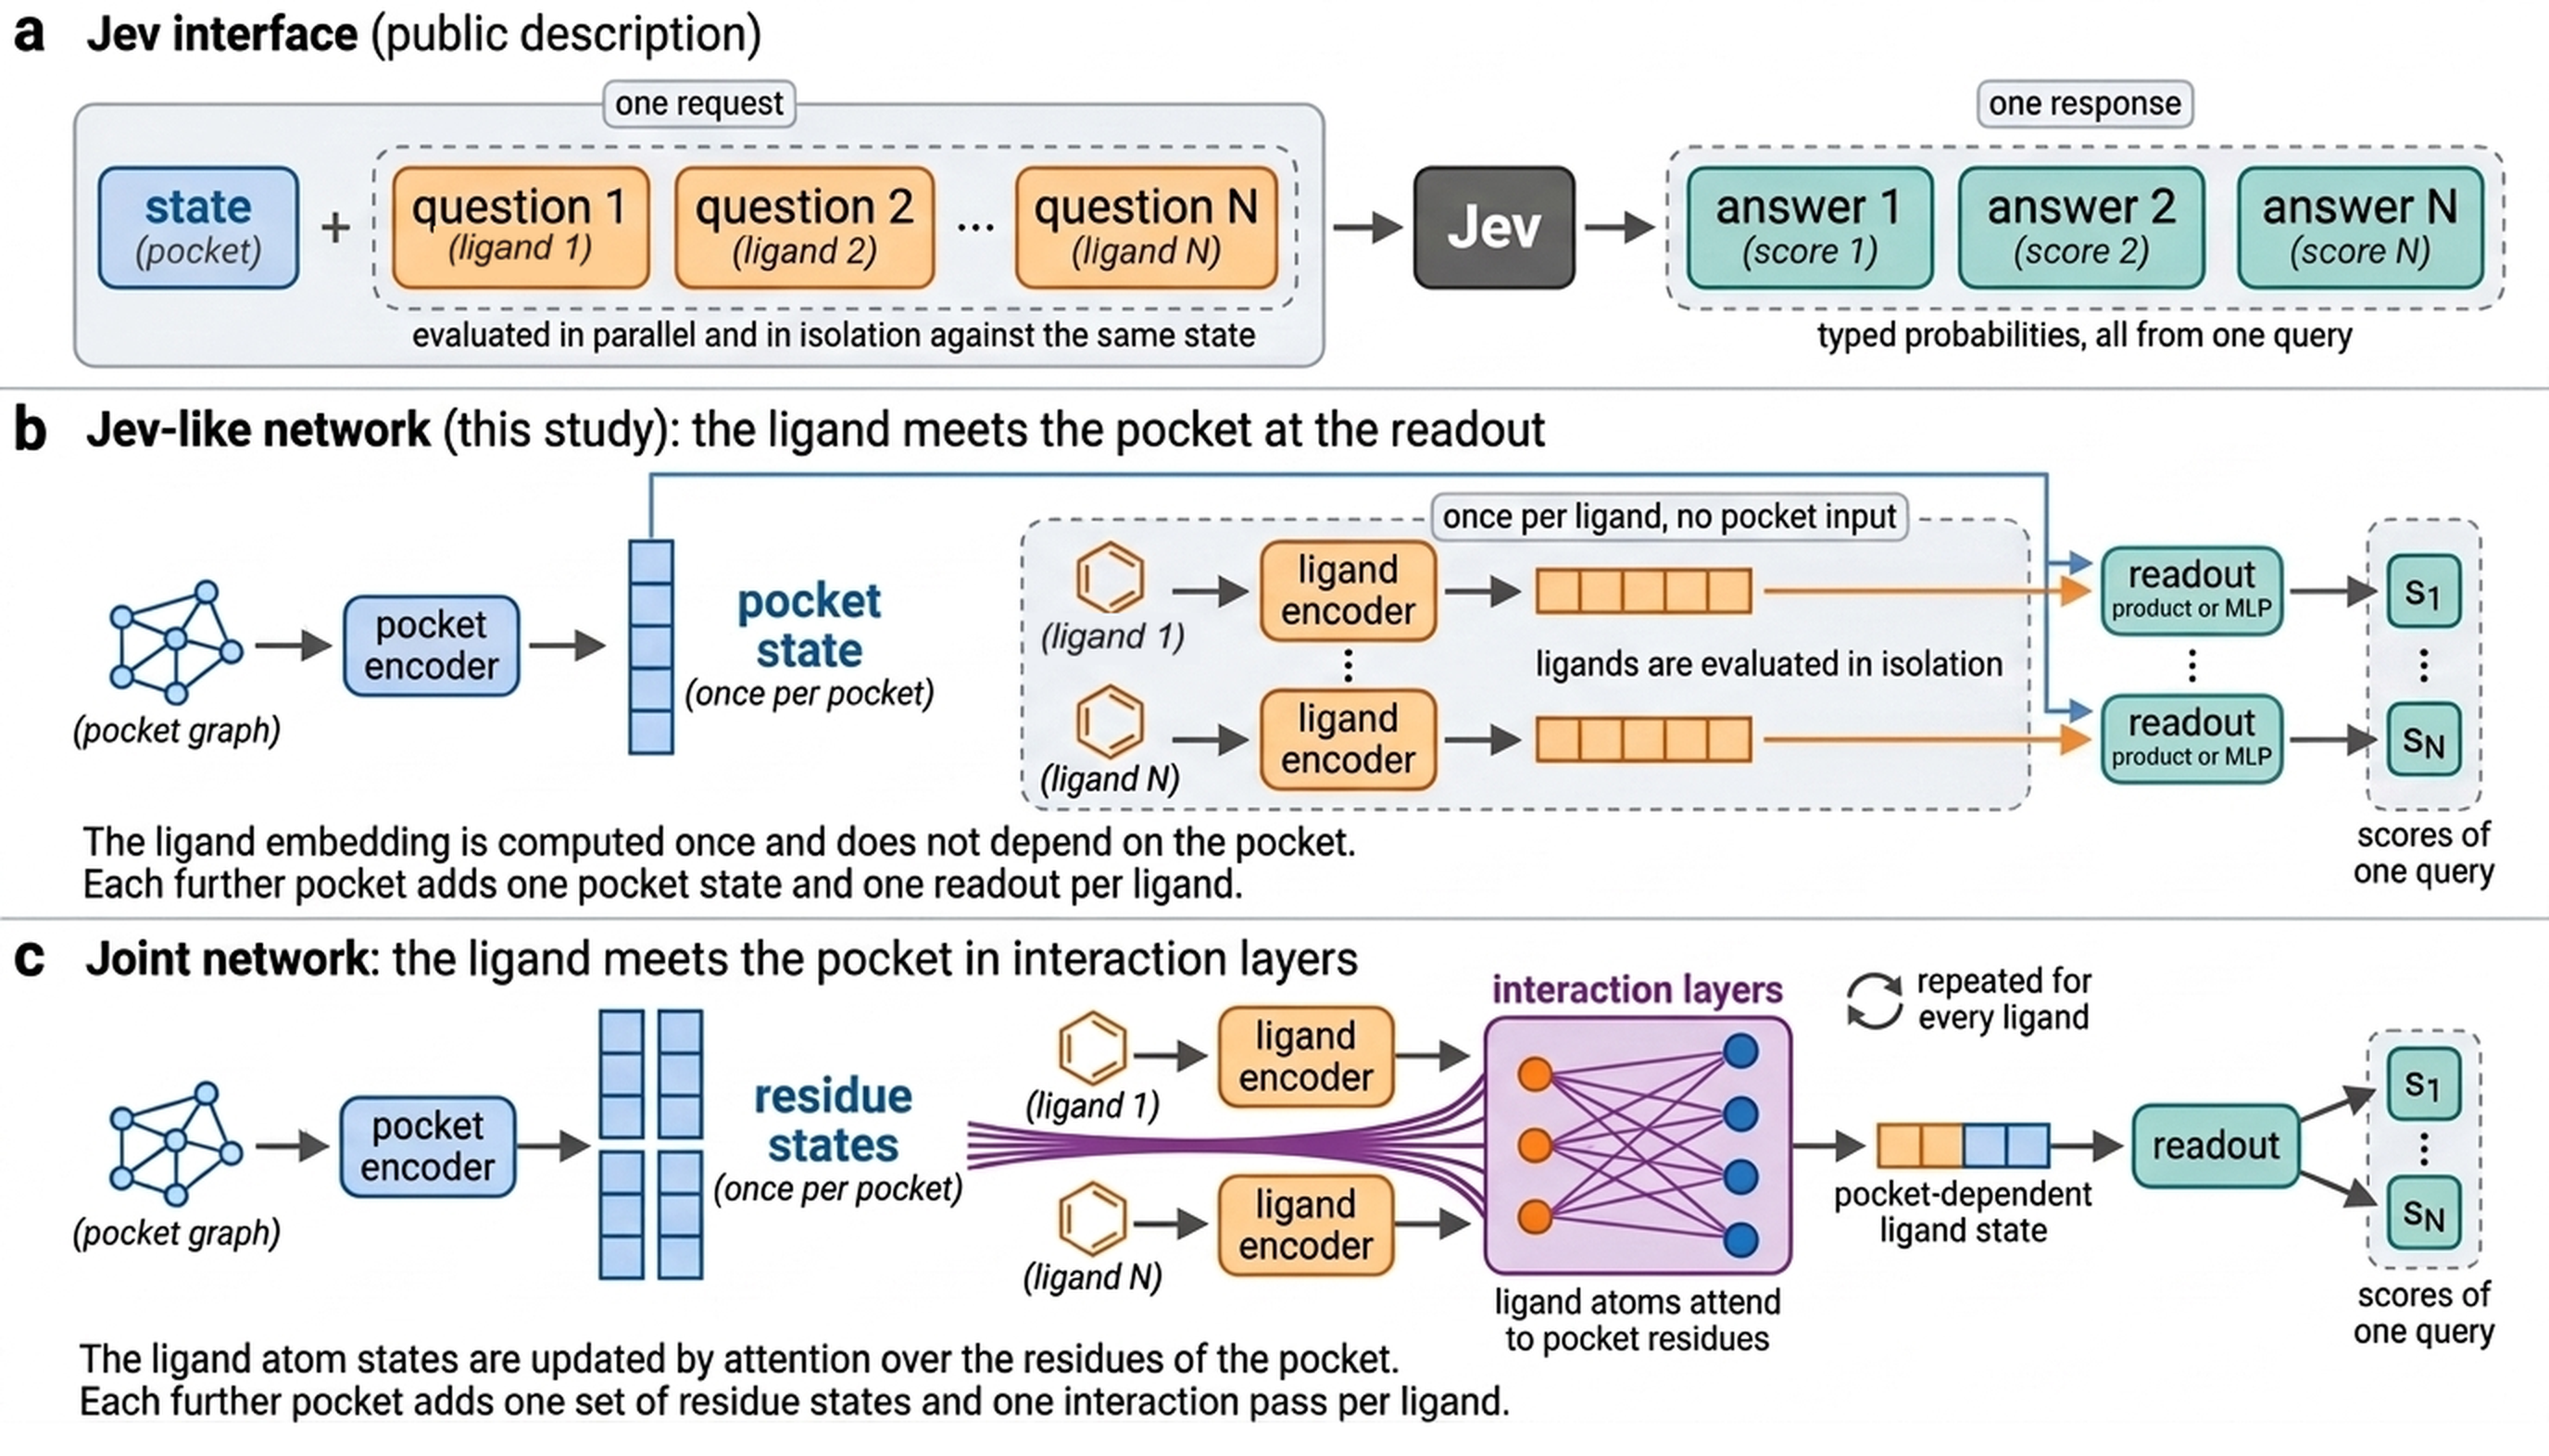
\includegraphics[width=\linewidth]{figures/fig1_concept}
\caption{The Jev interface and the two organizations of the surrogates. (a) Jev takes one state and several typed questions in one request, evaluates the questions in parallel and in isolation against the same state, and returns all answers in one response; the grey words in parentheses give the counterpart in this study. Blue marks the state, orange the questions and teal the answers, and the same colors mark the pocket, the ligands and the scores in b and c. (b) The Jev-like network encodes the pocket once into a cached state, embeds every ligand independently of the pocket and of the other ligands, and meets the pocket only at a cheap readout (a product of the pooled vectors for the dual encoder, a multilayer perceptron on the pooled vectors for the pooled network), so that each new pocket adds one pocket state and one readout per ligand. (c) In the joint cross-attention network the ligand atoms attend to the residues of the pocket in interaction layers, so that each new pocket adds one set of residue states and one interaction pass per ligand. The scores of all pairs rank the library for each pocket, and the best 10\% of the ranking are docked.}
\label{fig:concept}
\end{figure}


\section{Methods}

\subsection{Targets, ligands and splits}

We used the DOCKSTRING dataset, which holds AutoDock Vina scores of 260,155 drug-like ligands docked into 58 prepared receptors.\cite{dockstring,vina} The scores come from the Vina 1.1.2 binary bundled with the DOCKSTRING package.\cite{dockstringrepo} Targets were grouped into 22 protein families. Entire families were assigned to one role, which gave 39 training targets, 10 development targets and 9 test targets. Ligands were grouped by Bemis-Murcko scaffold\cite{bemis1996} and split into a training set of 156,095 molecules and development, two calibration and test sets of 26,015 molecules each. No scaffold group occurs in two sets. The networks of the main text were trained on the docking scores of \kfFoldTrainMin{} to \kfFoldTrainMax{} of the \kfNTargets{} training and development targets, depending on the cross-fitted fold, with 40{,}000 training ligands per target. They were evaluated by screening new ligands against the known pockets of their training data, the pockets whose docking scores the network was trained on. A hit is a ligand in the lowest 1\% of the scores of a pocket within the ligand set that is evaluated. The evaluation ligands are 10{,}000 development ligands that were not used in training.
\subsection{Networks}

The pocket is a residue graph. Each node carries amino-acid identity, mean partial charge, the distribution of AutoDock atom types and distance features, and edges connect the 16 nearest residues with radial basis features of the distance. A three-layer message-passing encoder\cite{gilmer2017} turns this graph into residue embeddings. The ligand encoder is a three-layer message-passing network over the two-dimensional atom graph. Neither encoder sees coordinates of the ligand or a docking pose. The networks share these encoders (dimension 128) and differ in how they combine the ligand with the pocket. The dual encoder (\paramsDual{} parameters) scores the product of a ligand vector and a pooled pocket vector. The scoring of a screen against many pockets is therefore a matrix product, and the ligand embedding is independent of the pocket, so that the dual encoder is Jev-like. The cross-attention network (\paramsXa{} parameters) passes the ligand atom states through two cross-attention layers with four heads, in which the ligand atoms attend to the residues of the pocket. It reads the pooled result with a multilayer perceptron. The representation of a ligand therefore depends on the pocket, and every pair needs the interaction layers. A pooled-concatenation variant of the Jev-like network (\paramsPc{} parameters, the count of the dual encoder because the two readouts have as many weights) reads the concatenated pooled ligand and pocket vectors with a multilayer perceptron in place of the product. The constant-pocket network is the dual encoder trained with one synthetic pocket graph for every target, and the cross-fitted group also has constant-pocket versions of the pooled and cross-attention networks. Every network has a hit-probability readout, which ranks the ligands, and a score readout.

\subsection{Training}

Every network was trained with AdamW\cite{loshchilov2019} (learning rate $3\times10^{-4}$, weight decay $10^{-4}$) on batches of 256 ligands of one training pocket. The loss was the binary cross-entropy of the top-1\% hits of the training scores of the pocket plus 0.2 times a Huber loss on standardized scores. Training ran for at most 60{,}000 updates or 10 epochs. The hit-probability readout was evaluated every 6{,}094 updates, and training stopped after three evaluations without improvement. The cross-fitted networks were trained in five folds of whole protein families (the kinases; the nuclear receptors; the class A GPCRs, CYP450 and MAO-B; the aspartyl proteases, metalloproteases, serine proteases S1, NOS1 and PARP1; and PDE5A, PTGS2 and PTPN1) over the 49 training and development targets. A network of a fold was trained on the targets outside the fold with 40{,}000 training ligands per target. Its checkpoint was the evaluation point with the highest macro recall at the 10\% budget on six of these targets against 10{,}000 calibration ligands. This rule chooses the checkpoint on seen pockets. The cross-fitted dual encoder, pooled network and cross-attention network were trained with the real pockets and with one constant synthetic pocket for every target, with seed 11. The Supporting Information describes the networks whose checkpoint was chosen on new targets (the existing networks) and the longer training recipe.

\subsection{Evaluation on known pockets}

Every network ranked the 10{,}000 evaluation ligands for each pocket of its training data with its hit-probability readout. The evaluation ligands were not used in training or in the choice of the checkpoint of the cross-fitted networks. The top-1\% recall at a budget is the fraction of the hits of a pocket that lie in the best 1, 5, 10 or 20\% of its ranking. The recall of a pocket is the mean over the folds that train on the pocket (four of five). The reported values are macro means over the pockets. The 95\% intervals are percentile intervals from 5{,}000 bootstrap resamples of the pockets. The paired difference of two networks is the difference of their per-pocket recalls, resampled in the same way. Each cross-fitted network was also evaluated on the pockets of its held-out fold (Supporting Information).

\subsection{Cost at the full scale}

The cost was measured at the full scale on one \tmAGpu{} rented from RunPod (PyTorch 2.4.1,\cite{paszke2019} CUDA 12.4). All \tmALig{} ligands of the DOCKSTRING collection were screened from SMILES against 1, 5, 20 and 57 pockets (all prepared receptors except DRD2, whose search box exceeds the Uni-Dock grid limit), and against 1{,}000 pockets obtained by using the 57 pockets cyclically. Every copy is encoded and scored again. The stages are the featurization of the SMILES on \tmAProcs{} CPU processes, the collation of the batches, the embedding of the ligands on the GPU, the pocket states of all pockets, the scoring of all pairs and the selection of the best 10\% of the ligands of every pocket with \texttt{torch.topk}. The model time is the sum of the GPU stages. Each GPU stage was synchronized and timed twice, and the shorter time is reported. The dual encoder scores all pairs with one matrix product on the cached ligand and pocket vectors. The pooled network decomposes the first layer of its readout into a ligand term and a pocket term that are computed once and combined for each pair. The cross-attention network keeps the pocket-independent ligand atom states of the whole library on the GPU without padding and passes them through the interaction layers for each pocket with fused attention. It was timed in float32 and in float16 for the interaction layers and the readout. Every implementation was checked against the module forward on 2{,}000 ligands and five pockets (rank correlation of at least 0.9999 in float32 and 0.999 in float16). The Supporting Information gives every stage.

Uni-Dock 1.2.0\cite{unidock} was timed on one RTX 4090 rented from RunPod (driver 570.169), the GPU model of the network timing. The settings were the Vina scoring function, one output pose and the DOCKSTRING box of each receptor. The receptor of each of three targets (ABL1, MAOB and PTGS2) was docked against the first $n$ of 1,023 prepared ligands (\dockPrepOkFourK{} for the batches of 4,000), a random sample of the DOCKSTRING collection, where $n$ is the number of ligands per call. Every combination of search mode (detail, balance and fast) and batch size (160, 256, 1,000 and 4,000 ligands per call, 160 for the detail mode only) was timed. The rate is the number of ligands with a score divided by the wall time of the \texttt{unidock} process. The time that docking needs for a screen is the number of pairs divided by the median rate of the configuration with the highest rate. This time leaves out the preparation of the ligand files (protonation, embedding and PDBQT conversion), which the networks do not need. The time of the networks includes the featurization of the ligands from SMILES. The Uni-Dock authors recommend at least 10{,}000 ligands per call, above the largest batch that we timed. The rate rose with the batch size over the batches that we timed (Supporting Information).



\section{Results and Discussion}

\subsection{On known pockets the Jev-like network keeps most of the recall of the joint network}

At a budget of the best 10\% of the ranking, the dual encoder recovers \kfDualTen{} of the top-1\% docking hits of the \kfNTargets{} known pockets (95\% interval \kfDualTenLo{} to \kfDualTenHi{}) and the cross-attention network \kfXattnTen{} (\kfXattnTenLo{} to \kfXattnTenHi{}; Table~\ref{tab:known}). The cross-attention network recovers \kfDiffXattnDualTen{} (\kfDiffXattnDualTenLo{} to \kfDiffXattnDualTenHi{}) more of the hits than the dual encoder, and the dual encoder keeps \kfRatioDual{}\% (\kfRatioDualLo{} to \kfRatioDualHi{}) of its recall. A network with one constant dummy pocket for every target recovers \kfConstTen{} (\kfConstTenLo{} to \kfConstTenHi{}), the recall that the ligand alone supports. The pocket state adds \kfDiffDualConstTen{} (\kfDiffDualConstTenLo{} to \kfDiffDualConstTenHi{}) for the dual encoder and \kfDiffXattnXattnConstTen{} (\kfDiffXattnXattnConstTenLo{} to \kfDiffXattnXattnConstTenHi{}) for the cross-attention network. At the 20\% budget the two networks recover \kfDualTwenty{} and \kfXattnTwenty{}. A Jev-like variant with a learned readout in place of the product recovers \kfPooledTen{} (\kfPooledTenLo{} to \kfPooledTenHi{}) and keeps \kfRatioPooled{}\% of the recall of the cross-attention network, so that the result does not depend on the product readout.

The choice of the checkpoint matters more for the cross-attention network than for the Jev-like network. When the checkpoint is chosen on new targets, the dual encoder and the cross-attention network recover \kpDualTen{} and \kpXattnTen{} on the \kpNTargets{} training pockets of the existing networks, against \kpConstTen{} for the constant pocket, and the three networks with real pockets are within \kpSpreadTen{} of each other (Supporting Information). The checkpoint of the cross-attention network lies at update \kpXaBestLo{} to \kpXaBestHi{} with this rule, against \kfXaBestLo{} to \kfXaBestHi{} when the checkpoint is chosen on known pockets.
\begin{table}[t]
\caption{Top-1\% recall of the networks on the 49 known pockets for ligands that were not used in training, within a budget of the best 1, 5, 10 and 20\% of the ranking (macro mean over the pockets; 95\% interval from bootstrapping the pockets). Each network is the mean over the cross-fitted folds that train on a pocket, with the checkpoint chosen on known pockets. The constant-pocket network is the dual encoder trained with one dummy pocket for every target. The pooled network replaces the product of the dual encoder by a learned readout. Time: seconds from SMILES to scores for the 260{,}155 ligands of DOCKSTRING against 1{,}000 pockets on one RTX 4090 (cross-attention in float16). Percentages and differences in the text are computed from unrounded values. The recall of every network with the checkpoint chosen on new targets and with longer training is in the Supporting Information.}
\label{tab:known}
\centering
\footnotesize
\setlength{\tabcolsep}{3pt}
\begin{tabular}{lcccrr}
\toprule
Network & 1\% & 5\% & 10\% (95\% interval) & 20\% & Time (s) \\
\midrule
Dual encoder & 0.29 & 0.72 & 0.88 (0.85 to 0.90) & 0.96 & 43.5 \\
Cross-attention & 0.35 & 0.79 & 0.92 (0.90 to 0.93) & 0.98 & 197 \\
Constant pocket & 0.25 & 0.64 & 0.81 (0.76 to 0.85) & 0.93 & 43.5 \\
Pooled concatenation (Jev-like, learned readout) & 0.31 & 0.75 & 0.89 (0.87 to 0.91) & 0.97 & 44.1 \\
\bottomrule
\end{tabular}
\end{table}



\subsection{The cost of a screen with the Jev-like network hardly grows with the number of pockets}

The dual encoder embeds every ligand once, and the scoring of a pocket is a matrix product. A joint network pays its interaction layers for every ligand-pocket pair. Table~\ref{tab:cost} and Figure~\ref{fig:cost}a give the time to screen all \tmALig{} ligands of DOCKSTRING from SMILES to scores on one \tmAGpu{}, measured at the full scale. The dual encoder needs \tmADualFiftySevenFull{} s for 57 pockets and \tmADualThousandFull{} s for 1{,}000 pockets, of which \tmAFeat{} s is the featurization of the ligands on the CPU. One more pocket adds \tmADualPerPocketMs{} ms to its model time. The cross-attention network needs \tmAXaHalfFiftySevenFull{} s in float16 and \tmAXaSingleFiftySevenFull{} s in float32 for 57 pockets, and \tmAXaHalfThousandFull{} and \tmAXaSingleThousandFull{} s for 1{,}000 pockets. One more pocket adds \tmAXaHalfPerPocket{} s in float16 and \tmAXaSinglePerPocket{} s in float32. The cross-attention network therefore needs \tmARatioXaHalfFiftySevenFull{} to \tmARatioXaSingleFiftySevenFull{} times the time of the dual encoder for 57 pockets and \tmARatioXaHalfThousandFull{} to \tmARatioXaSingleThousandFull{} times for 1{,}000 pockets. Without the featurization, which every network needs, the ratios of the model times are \tmARatioXaHalfFiftySevenModel{} to \tmARatioXaSingleFiftySevenModel{} for 57 pockets and \tmARatioXaHalfThousandModel{} to \tmARatioXaSingleThousandModel{} for 1{,}000 pockets (Supporting Information).

Uni-Dock docks \dockRateFastest{} ligands per second in its fastest search mode, which puts the \pocketPairs{} million pairs of the library against 57 pockets at \pocketDockDaysFast{} GPU-days. The dual encoder ranks the same pairs in \tmADualFiftySevenFull{} s. Figure~\ref{fig:cost}b puts recall and time together. For 1{,}000 pockets the dual encoder has a recall of \kfDualTen{} at \tmADualThousandFull{} s and the cross-attention network a recall of \kfXattnTen{} at \tmAXaHalfThousandFull{} s in float16.

\begin{figure*}[t]
\centering
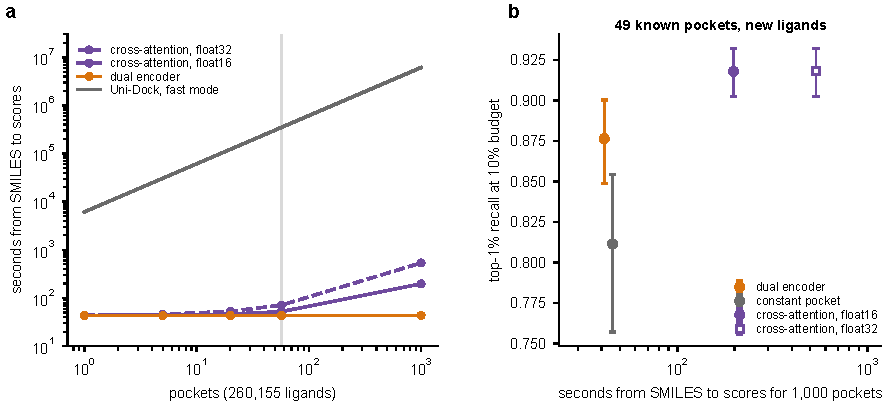
\includegraphics[width=\linewidth]{figures/fig_cost}
\caption{Cost and recall of the Jev-like and the joint network. (a) Time from SMILES to scores to screen the \tmALig{} ligands of DOCKSTRING against $P$ pockets on one \tmAGpu{}, measured at the full scale (markers), and the time of Uni-Dock in its fastest search mode (line). The vertical line marks the 57 pockets of DOCKSTRING, and the 1{,}000 pockets use them cyclically. (b) Top-1\% recall at the 10\% budget on the \kfNTargets{} known pockets for ligands that were not used in training (95\% intervals over the pockets) against the time for 1{,}000 pockets. The constant pocket is the dual encoder trained with one dummy pocket.}
\label{fig:cost}
\end{figure*}

\begin{table}[t]
\caption{Cost of screening the 260{,}155 ligands of DOCKSTRING at the full scale on one RTX 4090 (seconds, best of two runs for the GPU stages). Model time: ligand embedding, pocket states, scoring and selection of the best 10\% per pocket. End to end: model time plus the featurization of the SMILES on 32 CPU processes (39.3 s) and the collation of the batches. 1{,}000 pockets are the 57 pockets of DOCKSTRING used cyclically. Mpairs/s: million pairs per second of the scoring and selection stages for 57 pockets. Uni-Dock: library size times the number of pockets divided by the median docking rate at 4{,}000 ligands per call on one RTX 4090, without ligand preparation.}
\label{tab:cost}
\centering
\footnotesize
\setlength{\tabcolsep}{3pt}
\begin{tabular}{lrrrrr}
\toprule
 & \multicolumn{2}{c}{57 pockets} & \multicolumn{2}{c}{1{,}000 pockets} & Scoring rate \\
\cmidrule(lr){2-3}\cmidrule(lr){4-5}
Network & Model & End to end & Model & End to end & Mpairs/s \\
\midrule
Dual encoder & 1.61 & 43.3 & 1.81 & 43.5 & 19{,}314 \\
Pooled concatenation & 1.64 & 43.3 & 2.38 & 44.1 & 454 \\
Cross-attention, float16 & 10.4 & 52.0 & 156 & 197 & 1.69 \\
Cross-attention, float32 & 29.4 & 71.1 & 494 & 535 & 0.53 \\
Uni-Dock, fast mode & 349{,}204 & 349{,}204 & 6{,}126{,}390 & 6{,}126{,}390 & $4.2\times10^{-5}$ \\
Uni-Dock, detail mode & 1{,}037{,}358 & 1{,}037{,}358 & 18{,}199{,}267 & 18{,}199{,}267 & $1.4\times10^{-5}$ \\
\bottomrule
\end{tabular}
\end{table}



\subsection{Discussion}

The advantage of the Jev-like organization grows with the number of pockets. For 57 pockets the featurization of the ligands, which every network needs, dominates the time of the dual encoder, and the advantage over the cross-attention network is small. The organization therefore pays in the screen of a library against many pockets, where all pockets share the ligand embedding.

The price of the organization is a few points of recall at a budget of the best 10\% of the ranking. The dual encoder keeps \kfRatioDual{}\% of the recall of the cross-attention network. A shortlist of the best 10\% of the ranking costs a tenth of docking the library, so that the shortlist saves a factor of ten in the docking of the library at the recall of Table~\ref{tab:known}. The docked training sample of 40{,}000 ligands per pocket is \trainShareLib{}\% of the library, so the first screen of the library, with the sample and the shortlist docked, costs \shareLabelShortlist{}\% of docking the library, a saving of a factor of \factorLabelShortlist{}. Every further library that the networks screen saves the factor of ten.

The networks serve the pockets of their training data. They were trained on a docked sample of 40{,}000 ligands per pocket and rank new ligands against these pockets, which is the setting of a screen with a docked sample for every pocket of interest. For a pocket of a protein family outside the training data the networks have no target-specific knowledge to apply: in a cross-validation over protein families the pocket state adds no recall for the held-out family (Supporting Information). Such a pocket needs docking scores of its own before this organization can screen it.


\section{Conclusions}

A Jev-like network that encodes each pocket once into a shared state screens a library against many pockets at a cost that hardly grows with the number of pockets. On \kfNTargets{} known pockets the dual encoder keeps \kfRatioDual{}\% of the recall of a cross-attention network at a budget of the best 10\% of the ranking. It ranks \tmALig{} ligands against 57 pockets from SMILES in \tmADualFiftySevenFull{} s and against 1{,}000 pockets in \tmADualThousandFull{} s on one \tmAGpu{}, whereas the cross-attention network needs \tmARatioXaHalfThousandFull{} to \tmARatioXaSingleThousandFull{} times that time for 1{,}000 pockets and the docking of the 57 pockets takes \pocketDockDaysFast{} GPU-days in the fastest search mode of Uni-Dock.

\section{Data and Software Availability}

The code, the split definitions, the evaluation outputs and the timing records are in the GitHub repository \url{https://github.com/Gumgo91/jev-like-screening}. The trained checkpoints are in release v1.0 of the repository. The receptors and scores of the DOCKSTRING dataset are available from the DOCKSTRING repository and figshare under the Apache License 2.0. The docking benchmark used Uni-Dock 1.2.0\cite{unidock} and Open Babel\cite{openbabel} in the environment of \texttt{scripts/pod\_setup.sh}. The networks were trained on RunPod pods and on a desktop with one RTX 4060, and the timing ran on a RunPod pod with one RTX 4090 and on one with an L40S (PyTorch 2.4.1). The evaluation and analysis ran on a Windows workstation with Python 3.13.5, PyTorch 2.7.1,\cite{paszke2019} scikit-learn 1.7.1\cite{sklearn} and RDKit 2026.03.6\cite{rdkit}.

\section*{Notes}
The author declares no competing financial interest.

\begin{suppinfo}
The Supporting Information (PDF) describes the Uni-Dock benchmark, the stages of the full-scale timing, the existing networks, the longer training recipe of the cross-fitted networks, the evaluation on held-out protein families and the recall of every known pocket.
\end{suppinfo}

\begin{acknowledgement}
This research received no specific external funding. GPU time was rented from RunPod.
\end{acknowledgement}

\bibliography{refs}

\end{document}
